\documentclass[ngerman]{tudscrreprt}
\usepackage{selinput}
\SelectInputMappings{adieresis={ä},germandbls={ß}}
\usepackage[T1]{fontenc}
\usepackage{babel} 
\usepackage{isodate}
\usepackage{amssymb}
\usepackage{amsmath}
\usepackage{float} % lädt das Paket zur Verwendung von zusätzlichen Positionsbefehlen
\usepackage{wrapfig}  
\usepackage{picinpar}   
\usepackage{hyperref}

\begin{document}
\faculty{Fakultät Elektrotechnik und Informationstechnik} \department{} \institute{Institut für Regelungs - und Steuerungstheorie} \chair{Prof. Dr.-Ing. habil. Dipl. Math. Klaus Röbenack} \title{Analyse und Entwurf von Mehrgrößenregelung im Frequenzbreich\footnote{Mitschrift von Bolor Khuu}}
% \thesis{diss}
% \degree[Dr.-Ing.]{Doktor-Ingenieur}
\author{Prof. Dr.-Ing. habil. Dipl. Math. Klaus Röbenack}
% \dateofbirth{2.1.1990}
% \placeofbirth{Dresden}
\date{21.03.2014}
% \defensedate{20.10.2014}
% \referee{Dagobert Duck \and Mac Moneysac}
\maketitle
\tableofcontents
\newpage
\chapter{Mehrgrößensysteme in Zustandsraumdarstellung}
\section{Systembeschreibung}
Lineare Zustandsraummodelle \footnote{Mitschrift am 22.10.2014}
\begin{equation*}
\begin{matrix}
\dot x = A\,x + B\,u, \quad&A\in \mathbb{R}^{n\times n},&B\in \mathbb{R}^{n\times m}\\ 
     y = C\,x + D\,u, \quad&C\in \mathbb{R}^{r\times n},&D\in \mathbb{R}^{r\times m} 
\end{matrix}
\end{equation*}
Typisch:
\begin{itemize}
\item $m,r << n$ 
\item oft $m = r$
\item $D= 0$ kein Durchgriff
\end{itemize}
Lösung im Zeitbereich mit Anfangswert $x(0) = x_0 \in \mathbb{R}^{n}$
\begin{equation*}
\begin{matrix}
x(t) 	&=& e^{At}x_0 + \int\limits_{0}^{t}e^{A(t-\tau)}\cdot B u(\tau)d\tau &\\ 
		&=&\phi(t)x_0 + \int\limits_{0}^{t}\phi(t-\tau)B\,u(\tau)d\tau&\\ 
\phi(t) &=&e^{At} = \sum\limits_{k=0}^{\infty}\frac{(At)^{k}}{k!} \Rightarrow &\text{ Fundamentalmatrix}
\end{matrix}
\end{equation*}
\section{Kalmankriterium und Steuerbarkeitsindizus}
\subsection*{Definition} Ein System heißt vollständig (zustands).-steuerbar, wenn es von jedem Anfangszustand $\mathbf{x}(0)$ in endlicher Zeit $T>0$ durch geeignete Wahl des Eingangssignal $\mathbf{u}: [ 0,T] \rightarrow \mathbb{R}^{m}$ in einem beliebig vorgegebenen Endzustand $\mathbf{x}(t)$ überführt werden kann. 
\begin{figure}[H]
\centering
\def\svgwidth{200pt} 
  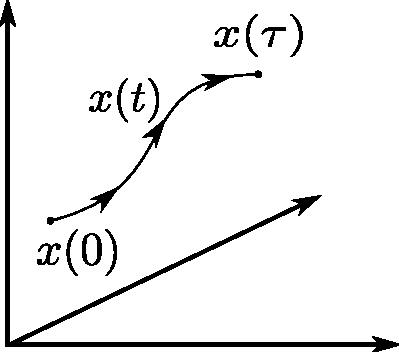
\includegraphics[width=3.7cm]{images/image1.pdf}
\end{figure}
Steuerbarkeitskriterien:
\begin{itemize}
\item Kalman
\item Hautus
\item Gilbert
\item Gram
\end{itemize}
\subsection*{Satz(Kalmanische Steuerbarkeitskriterium)}
Das System ist genau dann zustandssteuerbar, wenn die kalmanische Steuerbarkeitsmatrix\\ $Q_s = (B, AB,\dots, A^{n-1}B)$ den Rang $n$ besitzt. (voller Zeilenrang)
\begin{align*}
(\texttt{Matlab/Octave}):& Q_s = \texttt{ctrb}(A,B)\\
(\texttt{SciLab}):& Q_s =\texttt{cont$\_$mat}(A,B)
\end{align*}
SI(single-input, $m=1$): $Q_s \in \mathbb{R}^{n\times n}$, quadratisch, steuerbar $\iff$ $Q_s$ regulär (invertierbar)\\ 
MI(multi-input, $m>1$): $Q_s \in \mathbb{R}^{n\times nm}$, rechteckig, $n$-Zeilen, $nm$-Spalten \\ 
maximal $n$-Spalten können linear unabhängig sein. \\ 
\subsection*{Definition}Die kleinste Zahl $q$ mit \texttt{rang}$(B,AB,\dots, A^{q-1}B) = n$ heißt Steuerbarkeitsmatrix von $(A,B)$. \\ 
Umordnung/Auswahl der Spalten der Steuerbarkeitsmatrix
\begin{equation*}
Q_A = \left( b_1,Ab_1,\dots, A^{k_1 - 1}b_1, b_2, Ab_2,\dots, A^{k_2 - 1}b_2,\dots,b_m,Ab_m,\dots,A^{k_m-1}b_m \right) \quad \in \mathbb{R}^{m\times n}
\end{equation*}
Auswahlmatrix mit Rang $Q_A = n, \quad \sum\limits_{i=1}^{m} k_i = n \qquad (k_1,\dots,k_m)\dots $Pseudosteuerbarkeitsindizes\\ 
Zusammenhang zum Steuerbarkeitsindex $q \le \max\limits_{1\le i\le m}^{} k_i$\\ 
\subsection*{Beispiel} \begin{equation*}
A = \begin{pmatrix}
1 & 0 & 1\\ 
0 & 2 & 3\\ 
0& 0 & 0
\end{pmatrix} , \qquad B =\begin{pmatrix} 1&0\\ 2&0\\ 0&1 \end{pmatrix} \qquad
\begin{matrix}
\left. \begin{matrix} \text{rang}B &=& 2\\ \text{rang}(B,AB) &=& 3 \end{matrix}\right\} \text{steuerbar und } q= 2 & \qquad \\ 
\text{rang}(A,AB,A^2B) = 3& 
\end{matrix}
\end{equation*}  
\subsection*{Ziel} möglichst gleichmäßige Aufteilung der Indizes bzw. Eingänge\\
Mögliche Steuerbarkeitsindizes $(0,3), (1,2), (2,1), (2,1), (3,0)$
\begin{equation*}
\begin{matrix}
\text{Indizes:}& \text{Auswahlmatrix}& \text{Rang}\\ 
(0,3):& (b_2, Ab_2, A^2b_2) = \begin{pmatrix} 0&1&1\\1&5&10\\1&0&0\end{pmatrix}& 3\\ 
(1,2):& (b_1, b_2, b_2 A) = \begin{pmatrix} 1&0&1\\2&1&5\\0&1&0\end{pmatrix}& 3\\ 
(2,1):& (b_1, Ab_1, b_2) = \begin{pmatrix} 1&1&0\\2&4&1\\0&0&1\end{pmatrix}& 3\\ 
(3,0):& (b_1, Ab_1, A^2b_1) = \begin{pmatrix} 1&1&1\\2&4&8\\0&0&0\end{pmatrix}& 2
\end{matrix}
\end{equation*}
Auswahl der ersten $n$ linear unabhängige Spaltenvektoren der Steuerbarkeitsmatrix (von links nach rechts) $Q_s = (B, AB, \dots)= (b_1,\dots, b_m, Ab_1,\dots, Ab_m,\dots).$ ggf. auch Vertauschung der Eingänge zuläßig. Diese Auswahl führt auf die Steuerbarkeitsindizes oder Kronecker Indizes.
\subsection*{Beispiel} (Fortsetzung):
% \begin{equation*}
% Q_s= (B,AB, A^2B) = 
% \bordermatrix{~ & B & AB & A^2B \cr
%               &1\quad 0 & 1\quad 1 & 1\quad 1 \cr
%               &2\quad 1 & 4\quad 5 & 8\quad 10\cr
%               &0\quad 1 & 0\quad 0 & 0\quad 0\cr
%               }
% \end{equation*}
% Rang $\Rightarrow 1\,2\,3\,3\,3\,3$
\begin{figure}[H]
\centering
\def\svgwidth{200pt} 
  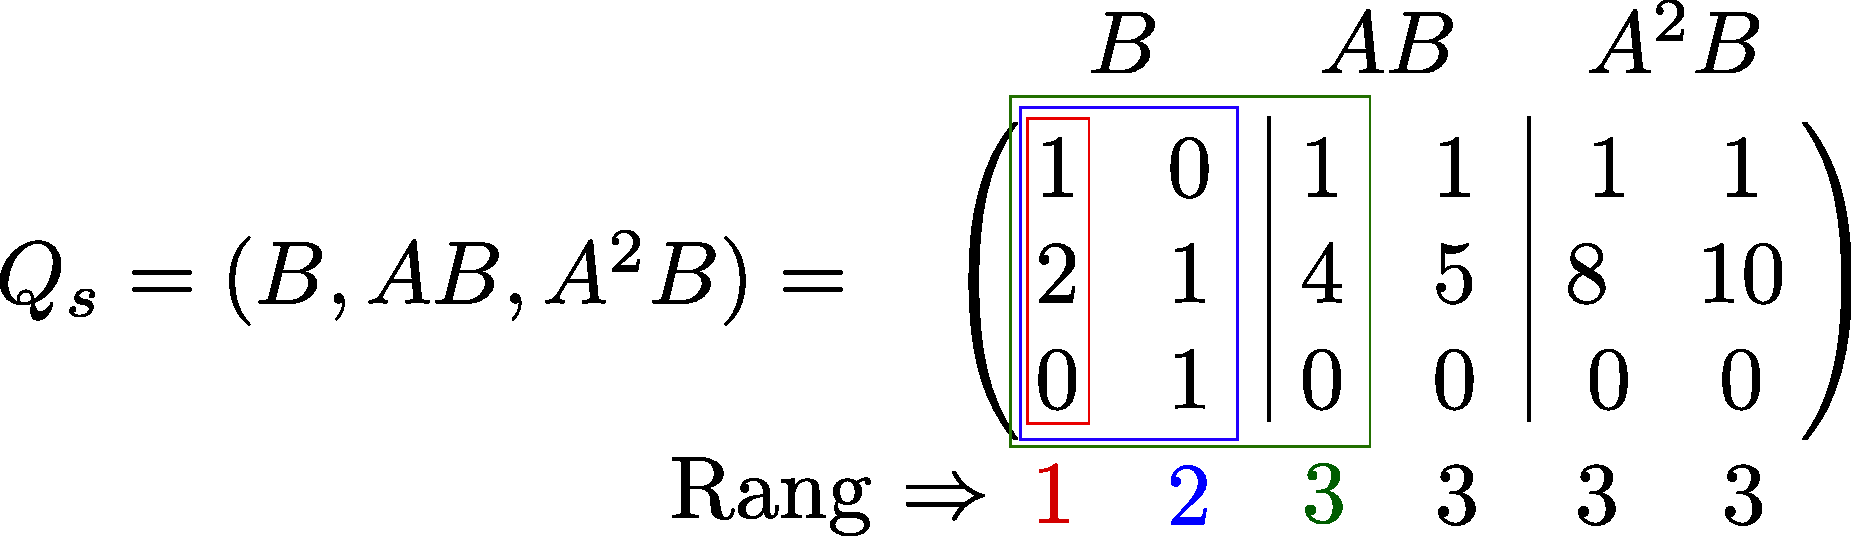
\includegraphics[width=7.7cm]{images/Zeichnung1.pdf}
\end{figure}

$Q_A = (b_1,Ab_1,b_2) \sim$ Steuerbarkeitsindizes $(2,1)$ \\ 
Vertauschung der Eingänge: $n_1 \iff n_2: \qquad \hat{B} = (b_2,b_1) = \begin{pmatrix} 0&1\\1&2\\1&0 \end{pmatrix}$  
\begin{figure}[H]
\centering
\def\svgwidth{200pt} 
  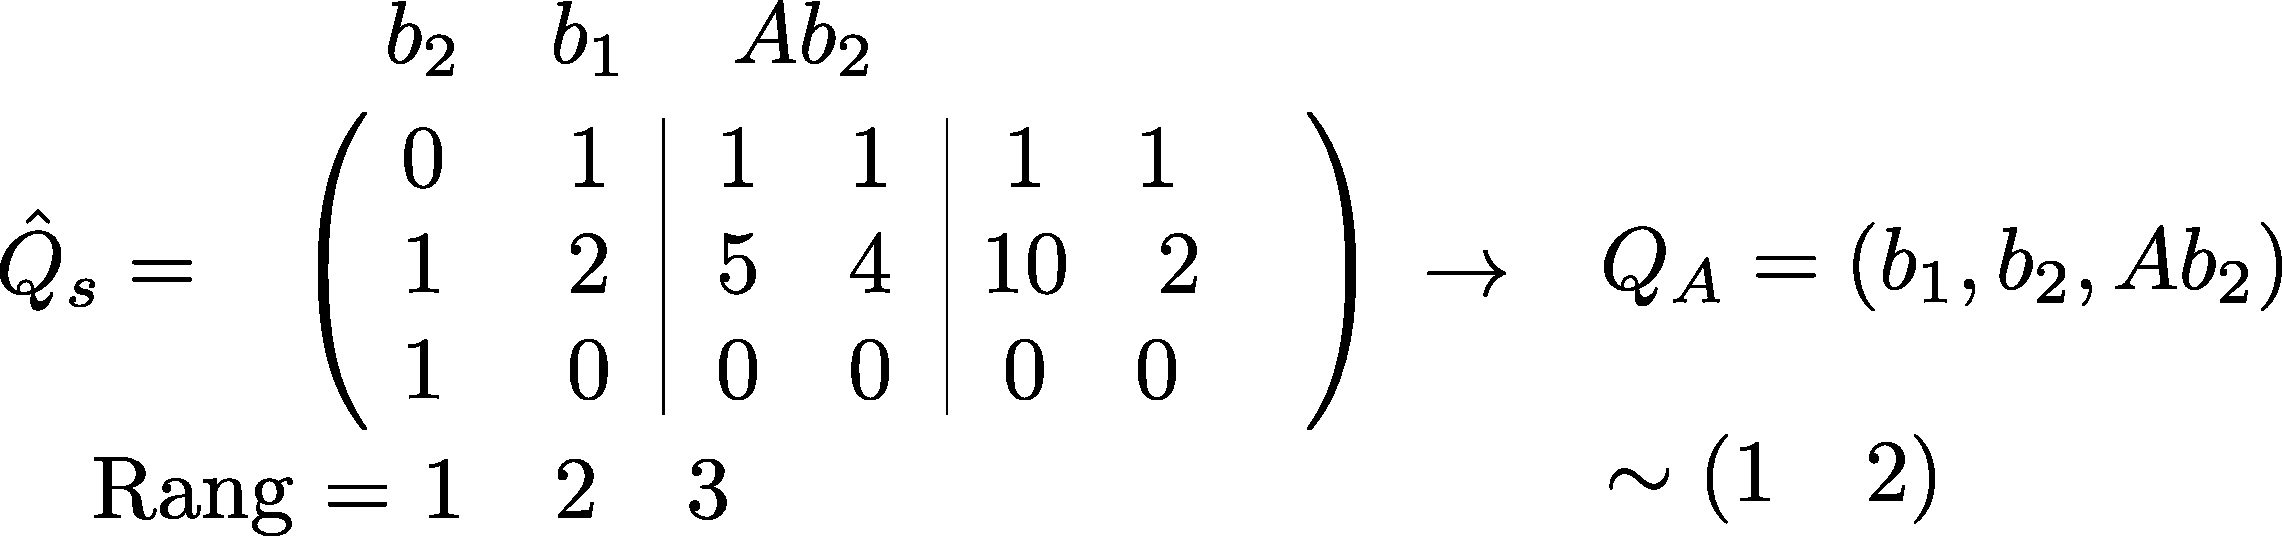
\includegraphics[width=9.7cm]{images/Zeichnung2.pdf}
\end{figure}
Steuerbarkeitsindizes: $(1,2), (2,1)$
\subsection*{Bemerkung}
\begin{itemize}
\item Steuerbarkeitsindizes kann bis auf Vertauschung eindeutig 
\item Vertauschung ist nicht immer möglich
\item Es gilt: $q = \max\limits_{1\le i\le m} k_i$
\end{itemize}
\section{Entwurf einer Zustandsrückführung mittels Regelungsnormalform}
Transformation des Originalsystems\footnote{Mitschrift am 29.10.2014}
\begin{equation*}
\dot x = Ax + Bu,\qquad A\in \mathbb{R}^{n\times n},\quad B\in\mathbb{R}^{n\times m}
\end{equation*}
in die Regelungsnormalform
\begin{equation*}
\dot{\bar{x}} = \bar{A}\bar{x} + \bar{B} u
\end{equation*}
% \begin{align*}
% \bar A =\left(\begin{array}{ c | c | c }
% \begin{matrix}
% 0 & 1 &   &  \\ 
%   &\ddots&\ddots &\\ 
%   &   & 0 & 1\\ 
% \star& \dots&\dots&\star 
% \end{matrix} & \begin{matrix} &&\\ &0& \\ &&\\ 
% \star&\dots& \star \end{matrix} &\begin{matrix} &&\\ &0& \\ &&\\ 
% \star&\dots& \star \end{matrix}\\ 
% \hline
% \begin{matrix} &&\\ &0& \\ &&\\ 
% \star&\dots& \star \end{matrix} &\begin{matrix}
% 0 & 1 &   &  \\ 
%   &\ddots&\ddots &\\ 
%   &   & 0 & 1\\ 
% \star& \dots&\dots&\star 
% \end{matrix}& \begin{matrix} &&\\ &0& \\ &&\\ 
% \star&\dots& \star \end{matrix}\\ \hline
% \begin{matrix} &&\\ &0& \\ &&\\ 
% \star&\dots& \star \end{matrix}&\begin{matrix} &&\\ &0& \\ &&\\ 
% \star&\dots& \star \end{matrix}&\begin{matrix}
% 0 & 1 &   &  \\ 
%   &\ddots&\ddots &\\ 
%   &   & 0 & 1\\ 
% \star& \dots&\dots&\star 
% \end{matrix}
% \end{array}\right)
% \end{align*}
\begin{figure}[H]
\centering
\def\svgwidth{200pt} 
  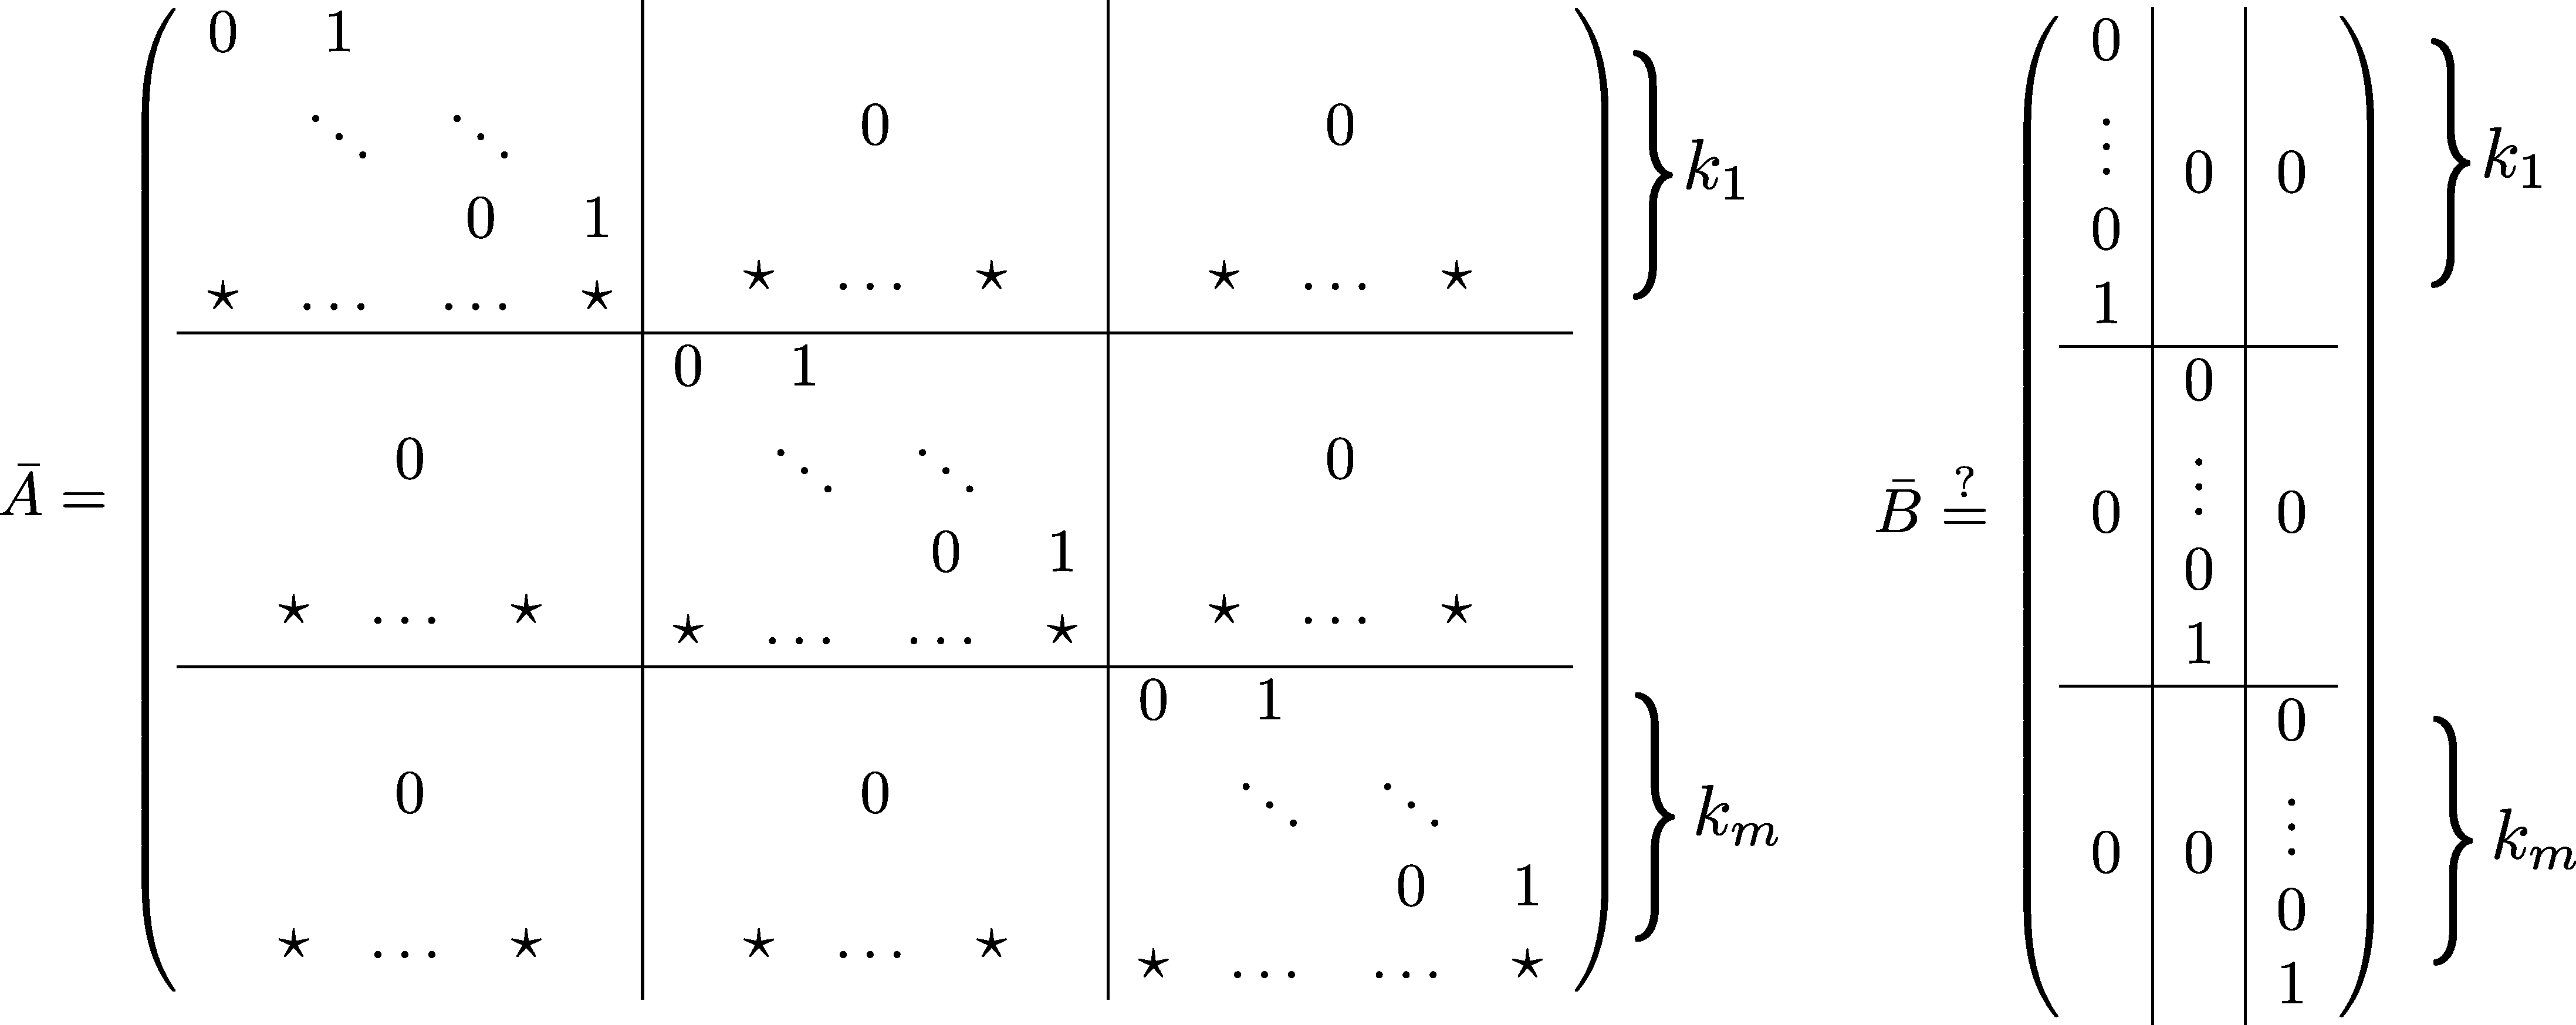
\includegraphics[width=16cm]{images/Amatrix.pdf}
\end{figure}
% \begin{align*}
% \bar B \overset{?}{=} \left(\begin{array}{ c | c | c }
% \begin{matrix}0\\\vdots\\0\\1
% \end{matrix} & 0 & 0 \\ 
% \hline 
% 0 & \begin{matrix}0\\\vdots\\0\\1
% \end{matrix} & 0\\ \hline
% 0& 0& \begin{matrix}0\\\vdots\\0\\1
% \end{matrix}
% \end{array}\right)
% \end{align*}
Rückführung $\bar K \in \mathbb{R}^{m\times n}$ mit 
\begin{align*} \bar A - \bar B \bar K = \bar A - 
\left(\begin{array}{c | c | c }
\begin{matrix} 0\\ \bar k_{11} \end{matrix} 
&
\begin{matrix} 0\\ \star \end{matrix}
&
\begin{matrix} 0\\ \bar k_{1m} \end{matrix}\\
\hline
\star & \star & \star \\
\hline 
\begin{matrix} 0\\ \bar k_{m1} \end{matrix} & \begin{matrix} 0\\ \star \end{matrix} & \begin{matrix} 0\\ \bar k_{mm} \end{matrix}
\end{array}\right)\\ \overset{!}{=} 
\left(\begin{array}{ c | c | c }
\begin{matrix} 0 & 1 & &&\\ &\ddots&\ddots&\\-p_{1,0}&\dots& \dots&-p_{1,p-1} \end{matrix} & 0 & 0 \\ 
\hline 
0 & \begin{matrix} 0 & 1 & &&\\ &\ddots&\ddots&\\\star&\dots&\dots &\star\end{matrix} & 0\\ \hline
0& 0& \underset{\text{Frobenius Regelmatrix}}{\begin{matrix} 0 & 1 & &&\\&\ddots&\ddots&\\\star&\dots& \dots&\star \end{matrix}}
\end{array}\right)
\end{align*} Koeffezienten der gewünschten charakteristischen Polynome. \\ 
Transformation: \begin{align*} \bar x &= T\,x ,\qquad T\in \mathbb{R}^{n\times n}\\ 
\dot{\bar{x}} & = T\,\dot x = T(Ax + Bu)\\ 
&= \underbrace{TAT^{-1}}_{\bar A} \bar x + \underbrace{TB}_{\bar B}u\end{align*} 
\begin{enumerate}
\item Ansatz für Zustandsrückführung $ u = -\bar k \bar x = -\underbrace{\bar k T}_{k} x$\\ 
Transformationsmatrix 
\end{enumerate}
% \begin{align*}
% T = \left(
% \begin{array}{ c }
% t_{1,1}^T \\ \vdots\\ t_{1,k_1}^T\\ \hline \vdots  \\ \hline t_{m,1}^T\\ \vdots\\ t_{m,k_m}^T
% \end{array}
% \right)
% \end{align*}
\begin{figure}[H]
\centering
\def\svgwidth{200pt} 
  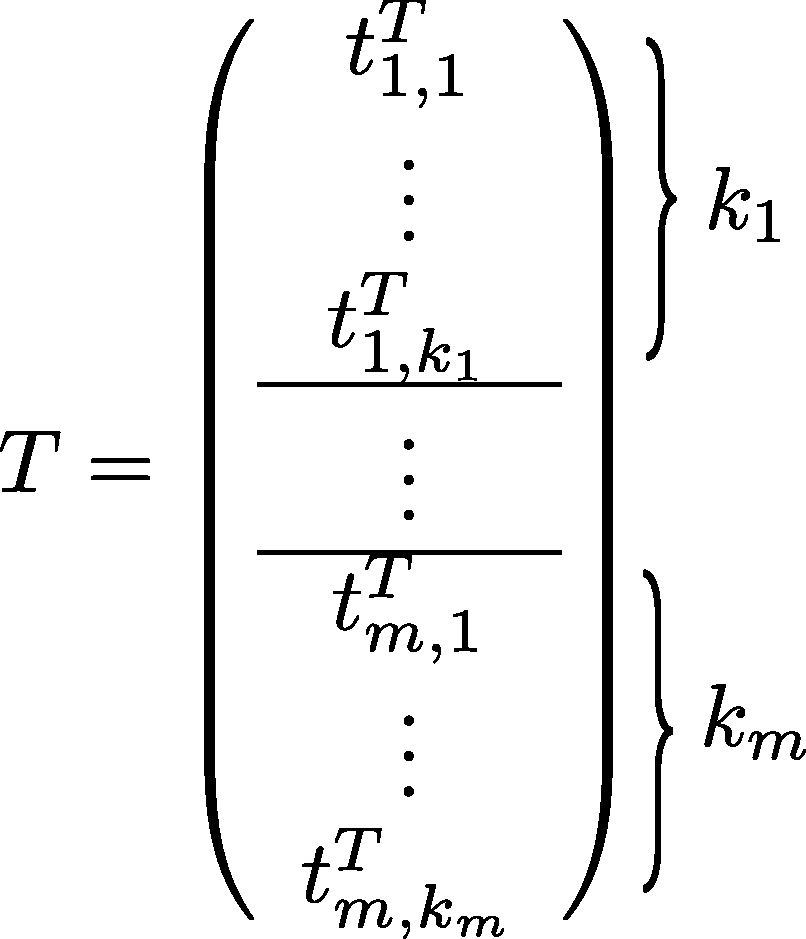
\includegraphics[width=3cm]{images/Tmatrix.pdf}
\end{figure} Ähnlichkeitstransformation $TAT^{-1} = \bar A \iff TA = \bar A T$
\begin{align*}
\left(
\begin{array}{ c }
t_{1,1}^T \\ t_{1,2}^T \\ \vdots\\ t_{1,k_1}^T\\ \hline \vdots
\end{array}\right)\cdot A = \left(
\begin{array}{ c | c }
\begin{matrix}
0&1 && \\ 
& \ddots&\ddots&\\
&&0&1\\ 
\star&\dots&\star& \star
\end{matrix}& \dots \\ \hline \vdots& \ddots
\end{array}
\right)\cdot \left(
\begin{array}{ c }
t_{1,1}^T \\ t_{1,2}^T \\ \vdots\\ t_{1,k_1}^T\\ \hline \vdots
\end{array}\right)
\end{align*}
Vergleich liefert $t_{i,j}^T \cdot A = t_{i,j+1}^T $ für $\substack{ i = 1,\dots, m\\ j = 1,\dots, k_i-1}$
\\ Transformationsmatrix \begin{align*}
T = \left(
\begin{array}{ c }
t_{1,1}^T \\ t_{1,1}^T\cdot A\\ \vdots\\ t_{1,1}\cdot A^{k_1 -1}\\ \hline \vdots\\ \hline t_{m,1}^T\\ t_{m,1}\cdot A\\ \vdots\\ t_{m,1}^T\cdot A^{k_m-1}
\end{array}
\right)
\end{align*} noch zu bestimmen \begin{align*} \begin{matrix} t_{1,1}^T =: t_1^T\\ \vdots\\ t_{m,1}^T =: t_m^T\end{matrix}\end{align*} 
Forderung am Eingangsmatrix: 
% \begin{align*}
% TB = \bar B = \left(
% \begin{array}{ c | c | c }
% \begin{matrix} 0 \\ \vdots\\ 0\\1 \end{matrix} & 0 & 0\\ \hline 
% 0& \begin{matrix} 0 \\ \vdots\\ 0\\1 \end{matrix} & 0 \\ \hline 
% 0 & 0& \begin{matrix} 0 \\ \vdots\\ 0\\1 \end{matrix}
% \end{array}
% \right)
% \end{align*}
\begin{figure}[H]
\centering
\def\svgwidth{200pt} 
  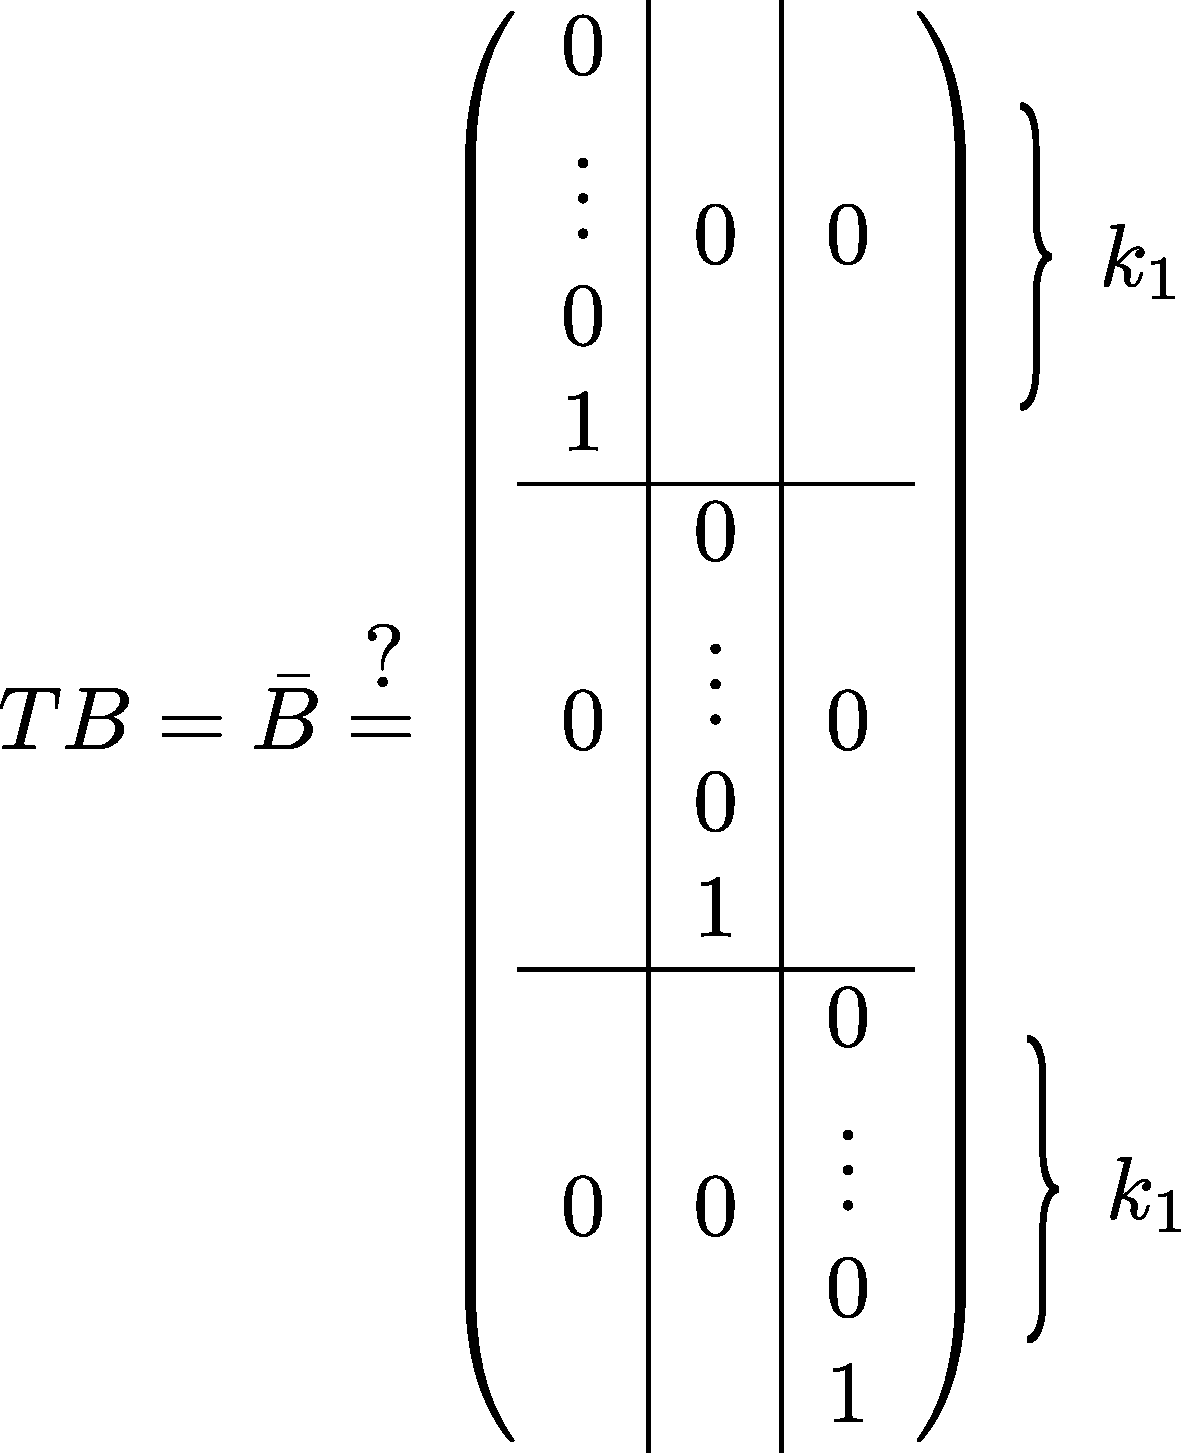
\includegraphics[width=4cm]{images/TBmatrix.pdf}
\end{figure}
Für einen Block \begin{align*}
\mathbb{R}^{k_i} \ni e_{k_i} = \begin{pmatrix} 
t_i^T\\ t_i^T\cdot A\\ \vdots\\ t_i^T\cdot A^{k_i -1} 
\end{pmatrix}\cdot b_i
\end{align*}
Zeilenweise für $i-$tes Teilsystem: \begin{align*}
t_i^T \cdot (b_i, Ab_i ,\dots, A^{k_i -1}b_i ) = e_{k_i}^T
\end{align*}
Simultan für alle in Teilsysteme 
\begin{align*}
\begin{pmatrix}
t_1^T\\ \vdots\\ t_m^T
\end{pmatrix} \underbrace{
(b_1,Ab_1,\dots, A^{k_1 -1} b_1, \dots, b_m, Ab_m, A^{k_m-1}b_m)
}_{Q_A \dots \text{ Auswahlmatrix}}
= \begin{pmatrix} e_{v_1}^T\\ \vdots\\ e_{v_m}^T\end{pmatrix}
\end{align*} mit \begin{align*} v_1 &= k_1\\ v_2&= k_1 + k_2\\ &\vdots\\ v_m&= k_1 + \dots + k_m \end{align*} \begin{align*}
\iff \begin{pmatrix}
t_1^T\\ \vdots\\ t_m^T 
\end{pmatrix} = \begin{pmatrix} e_{v_1}^T\\ \vdots\\ e_{v_m}^T \end{pmatrix} \cdot Q_A
\end{align*} 
\subsection*{Beispiel (Fortsetzung)}
\begin{align*}
A = \begin{pmatrix}
1 & 0 & 1\\ 0 & 2 & 3\\ 0 & 0 & \end{pmatrix}, \quad B = \begin{pmatrix} 1 & 0\\ 2 & 1\\ 0 & 1\end{pmatrix}
\end{align*}
Steuerbarkeitsmatrix \begin{align*}
Q_s = \left( B, AB, A^2B \right) = \left( \begin{array}{ c | c | c }
\begin{matrix} 1 & 0\\ 2 & 0\\ 0 & 1\end{matrix} & \begin{matrix} 1 & 1 \\ 4 & 5\\ 0& 0 \end{matrix} & \begin{matrix} 1 & 1\\ 8 & 10\\ 0 & 0 \end{matrix}
\end{array}\right)
\end{align*}
Auswahlmatrix zu Steuerbarkeitsindizes $k_1 = 2, k_2 = 1: $ \begin{align*}
Q_A = (b_1, Ab_1, b_2 ) = \begin{pmatrix} 1 & 1 & 0\\ 2 & 4 & 1\\ 0 & 0 & 1\end{pmatrix} \end{align*}
\begin{enumerate}
\item Aufstellen der Steuerbarkeitsmatrix $Q_s$ 
\item Bestimmung der Steuerbarkeitsindizes (Aufstellen Auswahlmatrix $Q_A$)
\begin{align*}
\begin{matrix} k_1 = 2\\ k_2 = 1 \end{matrix}, \quad Q_A = (b_1, Ab_1, b_2) = \left(\begin{array}{c | c }
\begin{matrix} 1 & 1\\ 2& 4\\ 0& 0 \end{matrix} & \begin{matrix} 0 \\ 1\\ 1\end{matrix}
\end{array}\right)
\end{align*}
\item Bestimmung der blockweise ersten Zeilenvektoren $t_1^T, \dots, t_m^T$ der Transformationsmatrix 
\begin{align*}
v_1 &= k_1 = 2\\ 
v_2 &= k_1 + k_2 = 3 
\end{align*}
\begin{align*}
\begin{pmatrix}
t_1^T\\ t_2^T 
\end{pmatrix} = \begin{pmatrix} e_{v_1}^T\\ e_{v_2}^T \end{pmatrix} \cdot Q_A^{-1} = \begin{pmatrix} 0 & 1& 0 \\ 0&0&1 \end{pmatrix} \cdot Q_A^{-1} =\begin{pmatrix} -1& 0.5& -0.5\\ 0 & 0 & 1\end{pmatrix}
\end{align*}
\item Aufstellen der Transformationsmatrix 
\begin{align*}
T = \left(\begin{array}{ c } 
t_{1,1}^T\\ t_{1,2}^T \\ \hline t_{2,1}^T
\end{array}\right) = \left(\begin{array}{ c } t_1^T\\ t_1^T\cdot A\\ \hline t_2^T\end{array}\right) = \left(\begin{array}{ c c c }
-1 & 0.5 & -0.5\\ -1 & 1 & 0.5\\ \hline 0 & 0 & 1
\end{array}\right)
\end{align*}
\item Transformation des Systems \begin{align*}
\bar A = TAT^{-1} = \left(\begin{array}{ c | c }\begin{matrix} 0 & 1 \\ -2& 3\end{matrix} & \begin{matrix} 0\\ -0.5 \end{matrix}\\ \hline \begin{matrix} 0 & 0 \end{matrix} & 0  \end{array}\right),\qquad \bar B = TB = \left(\begin{array}{ c | c } 
\begin{matrix} 0\\ 1 \end{matrix} & \begin{matrix} 0\\ 1.5\end{matrix} \\ \hline 0 & 1
\end{array}\right) ?
\end{align*}
Problem tritt nur bei verschiedenen Steuerbarkeitsindizes auf.\\ Allgemeine Form\begin{align*}
\bar B = 
\begin{array}{ c c }
\left(\begin{array}{ c | c | c } 
\begin{matrix} 0\\ \vdots\\ 0\\ 1 \end{matrix} & \begin{matrix} 0 \\ \star \end{matrix} & \begin{matrix} 0 \\ \star \end{matrix} \\ \hline \begin{matrix} 0 \\ \star \end{matrix} & \begin{matrix} 0\\ \vdots\\ 0\\ 1 \end{matrix} & \begin{matrix} 0\\ 1 \end{matrix} \\ \hline \begin{matrix} 0\\ \star \end{matrix} & \begin{matrix} 0\\ \star \end{matrix} & 
\begin{matrix} 0\\ \vdots\\ 0\\ 1 \end{matrix} 
\end{array}\right) & \begin{matrix}\leftarrow \text{Zeile } v_1 = k_1\\\\\\\\ \leftarrow \text{Zeile } v_2 = k_1 + k_2\\\\\\\\ \leftarrow \text{Zeile } v_m\end{matrix}
\end{array}
\end{align*}
Zusammenfassen der Zeilen $v_1, \dots, v_m$ \begin{align*}
\begin{pmatrix} t_1^T\cdot A^{k_1 - 1} \\ \vdots\\ t_m^T\cdot A^{k_m-1} \end{pmatrix}\cdot B =: V \in \mathbb{R}^{m \times m}
\end{align*}
\end{enumerate}
\begin{enumerate}
\item Korrektur durch Eingangstransformation \begin{align*}\tilde B := \bar B \cdot V^{-1} = TBV^{-1}=
\left(\begin{array}{ c | c | c }
\begin{matrix} 0\\ \vdots\\ 0\\1 \end{matrix} & 0 & 0 \\ \hline & \ddots & 0 \\ \hline 0 & 0 & 
\begin{matrix} 0\\ \vdots\\ 0\\1 \end{matrix}
\end{array}
\right) = (e_{v_1}, \dots, e_{v_m})
\end{align*}
\item Variante der Zustandsrückführung \begin{align*}
u & = -V^{-1}\cdot \bar K \bar x \\ 
& = -\underbrace{V^{-1} \cdot \bar K T }_{ k \in \mathbb{R}^{m\times n}}x
\end{align*}
\end{enumerate}
Blockweiser Ansatz für Reglerverstärkung $\bar K :$ \begin{align*}
\bar K = \left(
\begin{array}{ c | c | c } 
k_{11}^T & & k_{1m}^T \\ \hline \vdots&\ddots& \vdots\\ \hline \underbrace{k_{m,1}}_{k_1} & \dots& \underbrace{k_{m,m}^T}_{k_m}
\end{array}
\right) = \begin{pmatrix} k_1^T\\ \vdots\\ k_m^T \end{pmatrix} \in \mathbb{R}^{m\times n}
\end{align*}
Geschloßener Kreis (Beispiel $m=3$) \begin{align*}
\bar A = \tilde B \cdot \bar K = \left(\begin{array}{ c | c | c }
\begin{matrix} 0& 1 &&\\ & \ddots & \ddots & \\ && 0&1\\ &\dots a_{11}^T&\dots& \end{matrix} & \begin{matrix} 0\\ \\\\ \dots a_{12}^T \dots \end{matrix} & \begin{matrix} 0\\ \\\\ \dots a_{1m}^T \dots \end{matrix}\\ \hline & &  \\ \hline 
\begin{matrix} 0\\ \\\\ \dots a_{m1}^T \dots \end{matrix}& \begin{matrix} 0\\ \\\\ \dots a_{m2}^T \dots \end{matrix}& \begin{matrix} 0& 1 &&\\ & \ddots & \ddots & \\ && 0&1\\ &\dots a_{mm}^T&\dots& \end{matrix}
\end{array}
\right) - \left(\begin{array}{c | c | c } 
\begin{matrix} 0\\ k_{11}^T \end{matrix} & \begin{matrix} 0\\ k_{12}^T \end{matrix}&\begin{matrix} 0\\ k_{1m}^T \end{matrix}\\ \hline 
\begin{matrix} 0\\ k_{21}^T \end{matrix}& \begin{matrix} 0\\ k_{22}^T \end{matrix}& \begin{matrix} 0\\ k_{2m}^T \end{matrix}\\ \hline 
\begin{matrix} 0\\ k_{m1}^T \end{matrix}& \begin{matrix} 0\\ k_{m2}^T \end{matrix}& \begin{matrix} 0\\ k_{mm}^T \end{matrix}
\end{array}\right)
\end{align*}
Vorgabe für geschloßenen Kreis \begin{align*}
\bar A - \tilde B \bar K = \underbrace{\left(\begin{array}{ c | c | c }
\begin{matrix} 0 & 1 &&\\ & \ddots & \ddots &\\ \dots& p_1^T &\dots&\dots\end{matrix} & 0 & 0\\ \hline 
0 & \ddots & 0\\ \hline 
0 & 0 & \begin{matrix} 0 & 1 &&\\ & \ddots & \ddots &\\ \dots& p_m^T &\dots&\dots\end{matrix}
\end{array}\right)}_{ =: P}
\end{align*} mit $i-$ten Teilsystem \begin{align*}
\mathbb{R}^{k_i \times k_i} \ni \left(\begin{array}{ c } 
\begin{matrix} 
0 & 1 &&\\ &\ddots&\ddots & \\ &&0&1
\end{matrix} \\ \hline p_i^T
\end{array}\right) = \left(\begin{array}{c}
\begin{matrix} 0& 1 &&\\ &&&\\ &&0&1 \end{matrix} \\ \hline -p_{i,0}\qquad -p_{i,k_i-1}  
\end{array}\right)
\end{align*}
\begin{align*}
p_i^T = (-p_{i,0} \dots -p_{i,k_i-1})
\end{align*} charakteristische Polynom 
\begin{align*}
\text{CP}_i(s) = p_{i,0} + p_{i,1}s + \dots + p_{i,k_i-1}s^{k_i-1} + s^{k_i}
\end{align*}Entkopplung der Teilsysteme (=Nebendiagonal und Null): $a_{ij}^T - k_{ij}^T = 0^T$\\ 
Vorgabe der Wunschdynamik ($\equiv$ Haupdiaganolblöcke)
\begin{align*}
a_{ii}^T - k_{ii}^T \overset{!}{=} p_i^T\\ 
\iff k_{ii}^T = a_{ii}^T - p_i^T
\end{align*}Darstellung in Originalkoordinaten \begin{align*}
\dot x & = (A - BK)x\\ 
\dot{\bar x} &= T (A - BK)T^{-1} \cdot \bar x\\
&= (TA - \underbrace{ \underbrace{TB}_{\bar B}V^{-1} }_{\tilde B} \bar K )T^{-1} \bar x
\end{align*}
\begin{align*}
\begin{matrix}
\iff (TA - \tilde B \bar K)T^{-1} \\ 
\iff TA - \tilde B \bar K = pT 
\end{matrix}&\overset{!}{=} p
\end{align*}
Zeile $v_i$ \begin{align*} 
t_{i,k_i}^T \cdot A - \underbrace{k_i^T}_{i-\text{te Zeile }\bar K} = p_i^T\cdot T 
\end{align*}
\begin{align*}
\qquad \Rightarrow  \begin{matrix}k_i^T &=&t_{i,k_i}^T \cdot A - p_i^T \cdot T &\\ &=&t_i^T\cdot A^{k_i} + &\begin{pmatrix}
p_{i,0}\cdot t_i^T\\ p_{i,1}\cdot t_i^T A\\ p_{i,k_{i-1}}\cdot t_i^TA^{k_i-1}
\end{pmatrix}  \end{matrix}
\end{align*}
\begin{align*}
&=t_i^T(p_{i,0}\cdot I + p_{i,1}\cdot A + \dots + p_{i,k_i-1} \cdot A^{k_i -1} + A^k)\\ 
&=t_i^T \cdot \text{CP}_i(A)
\end{align*}Gesammtverstärkung 
\begin{align*}
K = V^{-1} \bar K = V^{-1} \begin{pmatrix} t_1^T \text{CP}_1(A)\\ t_m^T \text{CP}_m(A) \end{pmatrix}
\end{align*}
Verallgemeinerung der Ackermannformel für Mehrgrößensystem
\subsection*{Beispiel Fortsetzung \footnote{Mitschrift am 05.11.2014}}
\begin{enumerate}
\item Teilsystem: Eigenwertvorgabe $-1, -2$ 
\begin{align*}
\text{CP}_1(s) &= (s+1)(s+2)\\ 
&= s^2 + 3s + 2\\ 
k_1^T &= t_1^T \cdot \text{CP}_1(A)\\ 
&=(-1, 0.5, -0.5)(2I + 3A + A^2)\\ 
&=(-6, 6, 2.5)
\end{align*}
\item Teilsystem: Eigenwert $-3, \Rightarrow \text{CP}_2(s) = (s + 3)$
\begin{align*}
k_2^T &= t_2^T\cdot \text{CP}_2(A)\\ 
&= ( 0, 0, 1)(3I + A)\\ 
&= (0, 0, 3).\\ 
\Rightarrow \bar k = \binom{k_1^T}{k_2^T} &= \begin{pmatrix} -6, &6, & 2.5\\ 0, & 0,& 3 \end{pmatrix}\\ 
V&= \begin{pmatrix} 1 & 1.5\\ 0 & 1 \end{pmatrix}&
\end{align*}
Gesammtverstärkung: \begin{align*}
K = V^{-1}\cdot \bar K = \begin{pmatrix} -6 & 6 & -2\\ 0 & 0 & 3\end{pmatrix}
\end{align*}
\end{enumerate}
\section{Hautus - Kriterium und Stabilisierbarkeit}
System: \begin{align*} 
\dot x = A x + B u, \qquad &A\in \mathbb{R}^{n\times n}\\ &B \in \mathbb{R}^{n\times m}
\end{align*}
\subsection*{Satz (Hautus - Kriterium)} Das System (bzw. das Paar $(A,B)$) ist dann zustandssteuerbar, wenn $\forall s \in \mathbb{C} ,\text{rang} (sI - A, B) = n.$\\ 
\subsection*{Bemerkung:} 
\begin{enumerate}
\item Die Bedingung muss nur für Eigenwerte $s$, der Matrix $A$ überprüft werden.
\item Gilbert-Kriterium $(A,B)$ werden in der Jordan-Normalform $(\tilde A, \tilde B)$ betrachtet.
\end{enumerate}
\begin{align*}
(sI - \tilde A, \tilde B) = \left(
\begin{array}{ c | c | c | c }
\begin{matrix}
s-s_1 & -1\\ & s-s_1
\end{matrix} & 0 & 0&\begin{matrix} \dots\\ \star \dots \star \end{matrix} \\ \hline
0 & s - s_2 & 0 & \star \dots \star \\ \hline
0 & 0 & s- s_3 & \star \dots \star
\end{array}\right)\\
\text{Rangabfall in der letzten 3 Zeilen für $sI - \tilde A$ für $s = s_i$}
\end{align*}
Der Abfall bei $sI - \tilde A$ für einen Eigenwert $s_i$, muss durch Einträge in $\tilde B$ ausgeglichen werden. 
\subsection*{Forderung:} Ein System mit $k > 1$ Jordanblöcken des gleichen Eigenwertes kann $m$ dann steuerbar sein, wenn es mindestens $m \ge k$ Eingänge besitzt.
\subsection*{Definition:}Das Paar $(A, B)$ heißt stabilisierbar, falls $\forall s \in \mathbb{C} $ mit $\text{Re} (s) \ge 0, \quad \text{Rang} (sI - A, B) = n.$\\ 
Interpretation: Alle instabilen Eigenwerde und steuerbar. 
\subsection*{Kalman-Zerlegung nach Steuerbarkeit:}
Sei $q\cdot \text{rang} Q_s < n$, Dann existiert eine Zustandstransformation \begin{align*}
\tilde x = \binom{\tilde x_1}{\tilde x_2} = Tx, \qquad T\in \mathbb{R}^{n\times n}, \text{ regulär}
\end{align*} 
die das System in ein steuerbares und ein nicht steuerbares Teilsystem zerlegt. 
\begin{align*}
\binom{\dot{\tilde{x}}_1}{\dot{\tilde{x}}_2} = \underbrace{\begin{pmatrix}
\tilde A_{11} & \tilde A_{12}\\ 0 & \tilde A_{22}
\end{pmatrix}}_{\tilde A}
\binom{\tilde x_1}{\tilde x_2} + \underbrace{\binom{\tilde B_1}{0}}_{\tilde B}u\\ 
\tilde A_{11} \in \mathbb{R}^{q\times q}, \qquad \tilde B_1 \in \mathbb{R}^{q\times m}
\end{align*}
\begin{figure}[H]
\centering
\def\svgwidth{200pt} 
  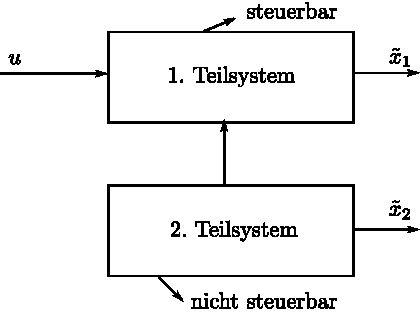
\includegraphics[width=6.7cm]{images/kalmanzerl.pdf}
\end{figure}
\begin{itemize}
\item $(\tilde A_{11}, \tilde B_{1})$ ist steuerbar
\item Eigenwerte \begin{align*}\texttt{eig }(A) &= \texttt{eig }(\tilde A)\\ &= \texttt{eig }(\tilde A_{11}) \cup \texttt{eig }(\tilde A_{22})\end{align*}
\item Das System ist dann stabilisierbar, wenn die Matrix $\tilde A_{22} $ stabil ist (d.h. alle Eigenwerte haben negativen Realteil). 
\item Zerlegung des Zustandsraumes: \begin{align*}
\mathbb{R}^n = \text{im} \underset{\substack{\text{Unterraum der}\\ \text{steuerbaren Zustände}}}{Q_s} \oplus \underset{\substack{\text{Unterraum der}\\ \text{unsteuerbaren Zustände}}}{\text{ker }Q_s^T}
\end{align*}
Transformationsmatrix 
\begin{align*}
T^{-1} = \left(\begin{array}{ ||| c |||}
\vdots
\end{array}\right)
\end{align*}
\begin{itemize}
\item $q$ Spaltenvektoren die im$ Q_s$ aufspannen.
\item $(n-q)$ Spalten (Komplement)
\end{itemize}
Seien $u_1, \dots, u_m \in \mathbb{R}^{m}$ die Spalten von $u = (u_1,\dots, u_m)$ und $v_1, \dots, v_n \in \mathbb{R}$ die Spalten von $v = (v_1, \dots, v_n)$ \\Dann : $M = uSv^T = \sum\limits_{i=1}^{r} \sigma_i \cdot \underbrace{u_i\cdot v_i^T}_{\text{dyad. Produkt}}$ 
\item Spalten $u_1, \dots, u_r$ spannen Bild der Matrix $M$ auf
\item Spalten $u_{r+1},\dots, u_m$ bilden Komplement ($u \dots$ orthogonal)
\end{itemize}
Transformationsmatrix: $Q_s \underset{\text{SVD}}{\rightarrow} u,S,v$ \begin{align*}
T^{-1} = u \iff T = u^{-1} \underset{\text{orthogonal}}{=} u^T
\end{align*}
\begin{align*}
\tilde x = Tx = u^T x \\ 
\dot{\tilde{x}} = T\dot x = T(Ax + Bu) &= TAT^{-1} \cdot \tilde x + TB u\\ 
&= \underbrace{u^T Au}_{\tilde A}\cdot \tilde x + \underbrace{u^TB}_{\tilde B} \cdot u
\end{align*}
\subsection*{Beispiel:}
Inverses Pendel auf Rädern\begin{align*}
\begin{pmatrix} \dot{\tilde x}_1\\ \dot{\tilde x}_2\\\dot{\tilde x}_3\\\dot{\tilde x}_4\\\dot{\tilde x}_5\end{pmatrix} = \left(\begin{array}{ c | c }
\begin{matrix} 0 & 0 & 1 & 0\\ 0 & 0 & 0 & 1\\ 0  &0 & 0& 0\\ 0 & a_{42} & 0 &0\end{matrix} & \begin{matrix} 0\\ 0\\ 0\\ 0\end{matrix} \\ \hline \begin{matrix} 0 & 1 & 0 & 0 \end{matrix} & 0
\end{array}\right) \cdot \begin{pmatrix} \tilde x_1\\ \tilde x_2\\\tilde x_3\\\tilde x_4\\\tilde x_5\end{pmatrix} + \begin{pmatrix} 0 \\ 0\\ 1 \\ b_4 \\ 0  \end{pmatrix} u \end{align*} 
\begin{itemize}
\item ohne $I$-Anteil $(n=4):$ steuerbar, rang$Q_s = 4$
\item mit $I$-Anteil $(n=5):$ nicht steuerbar, rang$Q_s = 4 < 5$
Begründung (Gilbert): doppleter Eigenwert bei 0. \begin{itemize} \item $2\times 2$ Block $\substack{\dot x_1 = 3\\ \dot x_3 = a}$
\item $1\times 1$ Block $I$-Anteil des Reglers \end{itemize} 
Für $s =s_0:$ Rangabfall 2 (in Hautus-Matrix), aber nur $m=1 $ Eingang. \\ 
$\tilde A_{22} = 0\Rightarrow$ nicht stabilisierbar.
\end{itemize}
\subsection*{Reglerentwurf für stabilisierbare Systeme:} 
\begin{enumerate}
\item Kalman-Zerlegung nach Steuerbarkeit
\begin{align*}
\binom{\dot{\tilde{x}}_1}{\dot{\tilde{x}}_2} = \begin{pmatrix} \tilde A_{11} & \tilde A_{12}\\ 0 & \tilde A_{22} \end{pmatrix} \binom{\tilde x_1}{\tilde x_2} + \binom{\tilde B_1}{0} \cdot u
\end{align*}
\item Zustandsrückführung für steuerbares Teilsystem\\ 
$\Rightarrow$ liefert Verstärkung $\tilde K_1$ \\ 
\begin{align*}
\text{\texttt{Matlab/Octave:}} & \tilde K_1 = \texttt{place}(\tilde A_{11}, \tilde B_1, [\dots])\\ 
\text{\texttt{Scilab:}} & \tilde K_1 = \texttt{ppol}(\dots) \\ 
\Rightarrow \tilde K = (\tilde K_1 \underset{\substack{\text{keine Rückführung für }\\ \text{unsteuerbarer Teilsystem}}}{0})
\end{align*}
\item Zustandsrückführung in Originalkoordinaten
\begin{align*}
\tilde x= Tx = u^T x \qquad \text{bzw. } x = u\tilde x \\ 
u = -Kx = -\underbrace{Ku}\tilde x\Rightarrow \tilde K &= K\cdot u\\ K &= \tilde K u^{-1} = \tilde K u^T
\end{align*}
\begin{align*}
\texttt{Scilab: } \qquad K = -\texttt{stabil}(A,B, [\underset{\substack{\text{Eigenwerte für}\\ \text{steuerbares Teilsystem} }}{\dots}])
\end{align*}
\end{enumerate}
\subsection{Nullstellen und Smith-Normalform}
Zustandsraummodell {\footnote{Mitschrift am 12.11.2014}} \begin{align*}
\dot x &= Ax + Bu, \qquad A\in\mathbb{R}^{n\times n}\\ 
y &= Cx
\end{align*}
\subsection*{Hautus-Kriterium:} Das System bzw. Paar $(A,B)$ ist steuerbar, wenn \begin{align*}
\forall s \in \mathbb{C}: \qquad \text{rang }(sI - A, B) = n
\end{align*}
Das System bzw. das Paar $(A,C)$ heißt beobachtbar, wenn \begin{align*}
\forall s\in \mathbb{C}: \qquad \text{rang}\binom{sI-A}{C} = n
\end{align*}
\subsection*{Definition:} Eine Zahl $s_0 \in \mathbb{C}$ heißt 
\begin{enumerate}
\item Eingangs-Entkopplungsnullstelle (input-decoupling zero), falls \begin{align*} \text{rang }(s_0I - A, B) < n \end{align*} 
\item Ausgangs-Entkopplungsstelle (output-decoupling zero), falls \begin{align*}
\text{rang }\binom{s_0 I -A}{C} < n
\end{align*}
\item Eingangs-Ausgangs Entkopplungsnullstelle (input-output-decoupling zero), wenn sie sowohl Eingangs als auch Ausgangsentkopplungsnullstelle ist.
\end{enumerate}
\begin{itemize}
\item Eingangs-Entkopplungsnullstelle = nicht steuerbare Eigenwerte/Modi
\item Ausgangs-Entkopplungsnullstelle = nicht beobachtbare Eigenwerte/Modi
\item Eingangs-Ausgangs-Entkopplungsnullstelle = Eigenwerte, die weder steuerbar noch beobachtbar sind.
\end{itemize}
\subsection*{Beispiel:} 
\begin{align*}
A = \begin{pmatrix}
1 & 0 & 0\\ 0 & -2 & 0\\ 0 & 0 & -1 \end{pmatrix}, \qquad B = \begin{pmatrix} 1\\ 0\\ 1\end{pmatrix}\\ 
C = (1\quad 1\quad 0) 
\end{align*}
\begin{enumerate}
\item Eingangs-Entkopplungsnullstelle $s = -2\qquad $ $\Rightarrow$ stabilisierbar
\item Ausgangs-Entkopplungsnullstelle $s = -1\qquad $ $\Rightarrow$ detektierbar
\item keine 
\end{enumerate}
$\Rightarrow$ Gilbert-Kriterium\\ 
Lösung: \begin{align*} x(t) &= e^{At}x(0) + \int\limits_{0}^t e^{A(t-\tau)}B\cdot u(\tau)d\tau \\ 
&=\begin{pmatrix} e^t && \\ & e^{-2t} &\\ &&e^{-t} \end{pmatrix} x(0) + \int\limits_{0}^t\begin{pmatrix} e^{t-\tau}\\ 0\\ e^{-(t-\tau)}\end{pmatrix} u(\tau) d\tau
\end{align*}
$\Rightarrow$ nur steuerbare Eigenwerte erscheinen in $e^{At} B.$\\ 
Ausgang: 
\begin{align*}
y(t) = C x(t) &= C e^{At} + \int\limits_0^t C\cdot e^{A(t-\tau)}Bu(\tau) d\tau \\ 
&= (e^{t}, e^{-2t}, 0)\cdot x(0) + \int e^{t-\tau} d\tau 
\end{align*}
$\Rightarrow$ nur beobachtbare Eigenwerte erscheinen in $C e^{At}$\\ 
$\Rightarrow$ nur steuerbare und beobachtbare Eigenwerte erscheinen in $C e^{At} B$
\subsection*{Modifizierte Hautus-Bedingung:}
Das System bzw. das Paar $(A,B)$ ist stabilisierbar, wenn \begin{align*}
\forall s\in \mathbb{C} \qquad \text{mit  Re}(s)\ge 0: \quad \text{rang }(sI - A, B) = n
\end{align*}
Das System bzw. das Paar $(A,C)$ heißt detektierbar, wenn \begin{align*}
\forall s\in \mathbb{C} \qquad \text{mit  Re}(s)\ge 0: \quad \text{rang }\binom{sI-A}{C} = n
\end{align*}
\subsection*{Normalrang einer Polynommatrix $M$:}
\begin{align*}
\underset{s\in \mathbb{C}}{\text{max }} \text{rang} M(s)
\end{align*}
System mit in Ein.-und Ausgängen \begin{align*}
\dot x &= Ax + Bu, &A\in \mathbb{R}^{n\times n}, \qquad B\in \mathbb{R}^{n\times m}\\ 
y &= Cx, &C\in \mathbb{R}^{m\times n}
\end{align*}
Rosenbrock-Matrix
\begin{align*}
P(s) = \begin{pmatrix}
sI-A & -B\\ C & 0 \end{pmatrix} \in \mathbb{R}[s]^{(n+m)\times(n+m)} 
\end{align*}
Die Rosenbrock-Matrix habe den Normalrang $n+m$. Eine Zahl $s_0 \in \mathbb{C}$ heißt dann invariante Nullstelle 
\begin{align*}
\text{rang }\begin{pmatrix}
sI-A & -B\\ C & 0 \end{pmatrix} < n+m
\end{align*}
Berechnung: $\text{det }P(s) \overset{!}{=} 0.$
\begin{itemize}
\item Beziehung zu Entkopplungs-Nullstellen \\
Aus \begin{align*}
\text{rang }(sI-A,B) < n \quad \text{ folgt }\quad \text{rang }\begin{pmatrix}s_0I-A& -B\\ C&0\end{pmatrix} < n+m  
\end{align*} 
als \begin{align*}
\text{rang }\binom{s_I -A}{C} < n \quad \text{ folgt } \quad \text{rang }\begin{pmatrix} s_0I-A & -B\\ C & 0 \end{pmatrix} < n+m
\end{align*}
$\Rightarrow$ Entkopplungsnullstellen sind auch invariante Nullstellen
\item Beziehung zu Übertragungsfunktion \begin{align*}
G(s) = C(sI-A)^{-1}B
\end{align*}
Schur-Formel: \begin{align*}
\text{det}\left(\begin{array}{ c | c } 
A & B\\ \hline 
C & 0
\end{array}\right) = \text{det }(A)\cdot \text{det }(D-C\cdot A^{-1}B) \text{  für $A$ regulär}
\end{align*}
\begin{align*}
\text{det }P(s) = \text{det }\begin{pmatrix}sI-A & -B\\ C & 0\end{pmatrix} &=\text{det }(sI-A)\cdot \text{det }(0-C(sI-A)^{-1}(-B))\\ 
&= \text{det }(sI-A)\cdot \text{det }\underbrace{(C(sI-A)^{-1}B)}_{G(s)}
\end{align*}
\end{itemize}
$\Rightarrow$ Nullstellen der Übertragungsfunktion sind auch invariante Nullstellen.
\subsection*{Invarianzeigenschaften der inverianten Nullstellen}
\begin{enumerate}
\item reguläre Transformation des Eingangsvektors \begin{align*}
\begin{matrix}
\omega(t) &= V^{-1}u(t)\\ 
u(t)&= V\omega(t) \end{matrix} \Rightarrow (A,B) \to (A,BV)
\end{align*}
\item reguläre Transformation des Zustandsvektors 
\begin{align*}
\begin{matrix}
\tilde x(t) = Tx\\ 
x = T^{-1} \tilde x \end{matrix}
 \Rightarrow (A,B,C) \to (\underset{\substack{\text{Ähnlichkeits}\\ \text{-transformation}}}{TAT^{-1}},TB, CT^{-1})
\end{align*}
\item Zustandsrückführung \begin{align*}
u = -Kx + w \rightarrow (A,B) \to (A - BK, B) 
\end{align*} Beweis in 3.: Rosenbrock-Matrix des geschloßenen Kreises
\begin{align*}
P(s) = \begin{pmatrix} sI - (A-BK) & -B\\ C & 0\end{pmatrix} = \begin{pmatrix} sI-A & -B\\ C & 0 \end{pmatrix} \underbrace{\begin{pmatrix} I_n & 0 \\ -K & I_m \end{pmatrix} }_{\text{det}\equiv 1} 
\end{align*}
\end{enumerate}
Invariante Nullstellen werden durch unimodulare Transformation, die auf die Rosenbrock-Matrix angewendet werden, nicht verändert. 
\subsection*{Definition:} Eine quadratische Polynommatrix \begin{align*}
U(s) \in \mathbb{R}[s]^{n\times n}
\end{align*}heißt \textbf{unimodular}, falls det$(U) \in \mathbb{R} \setminus \{0\}$\\ 
(Determinante ist nicht Null und hängt nicht von $s$ ab).
\subsection*{Folgerung:} Sei $U$ unimodular, dann existiert Inverse $U^{-1}$ und die Inverse ist wieder eine Polynommatrix \begin{align*}
U^{-1} = \frac{1}{\underbrace{\text{det }U}_{\text{reelle Zahl}\ne 0}}\cdot \underbrace{\text{adj}(U)}_{Polynommatrix}
\end{align*}
\subsection*{Satz:} Sei $M \in \mathbb{R}[s]^{p\times m}$ mit Normalrang $r$. Dann existieren unimodulare Matrizen $U,V$ derart, dass \begin{align*}
U(s)M(s)V(s) = \wedge (s)
\end{align*}mit Diagonalmatrix 
\subsection*{Smith-Normalform:} \begin{align*}
\wedge = \left(\begin{array}{ c | c } 
\begin{matrix}\lambda_1(x) &&\\ & \ddots &\\ &&\lambda_r(s) \end{matrix} & 0 \\ \hline 0 & 0
\end{array}\right) \in \mathbb{R}[s]^{p\times m}
\end{align*}mit monischen (monic) Polynome $\lambda_1,\dots, \lambda_r \in \mathbb{R}[s]$ wobei $\lambda_1| \lambda_2| \dots| \lambda_r.$\\ 
monisch $\dots$ höchster Koeffizient ist 1.
\begin{itemize}
\item Anwendung auf Rosenbrock-Matrix \footnote{Mitschrift am 26.11.2014}
\begin{align*}
P(s) &= \begin{pmatrix} sI-A & -B\\ C & 0 \end{pmatrix}\\ \text{det }(U(s)\cdot P(s)\cdot V(s))&=\underbrace{\text{det }U(s)}_{\text{konst}}\cdot \text{det }P(s) \cdot \underbrace{\text{det }P(s)}_{konst}\\ &=\text{det }\wedge = \lambda_1(s) \dots \lambda_r(s) =: \rho(s) \text{ für Normalrang } r=n+m
\end{align*}
\end{itemize}
\subsection*{Folgerung:} Die invariante Nullstellen sind die Nullstellen von $\rho(s)$\\ 
$\Rightarrow $erlaubt allgemeine Definition der invarianten Nullstellen. (auch für rechteckige bzw. singuläre Rosenbrock-Matrizen). \\
Anwendung auf die Hautus-Matrizen liefert Eingangs.-bzw. Ausgangs-Entkopplungsnullstellen. 
\begin{itemize}
\item $(A,B) $ ist genau dann steuerbar, wenn die Hautus-Matrix $(sI_n - A, B)$ die Smith-Normalform $(I_n, 0)$ besitzt. 
\item $(A,C)$ ist genau dann beobachtbar, wenn $\binom{sI_n - A}{C} $ die Smith-Normalform $\binom{I_n}{0}$ besitzt. 
\end{itemize}
\subsection*{Beispiel:}\begin{align*}A = \begin{pmatrix} 0 & -1 & 1\\ 1 & -2& 1\\ 0 & 1& 1\end{pmatrix},\qquad B = \begin{pmatrix} 1& 0\\ 1&1\\ 1&2\end{pmatrix} \end{align*}
$\text{rang } Q_s = 2<3$ \begin{itemize}\item nicht steuerbar \item existiert \end{itemize}Eingangsentkopplungsnullstelle $n - \text{rang }Q_s = 1$
\subsection*{Kalman-Zerlegung}
\begin{align*}V^{-1} AV = \begin{pmatrix} -2 &&\\ & -1&\\ &&0\end{pmatrix}, \quad V^{-1}B = \begin{pmatrix}0 & 0\\ 0 & \star\\ \star& \star\end{pmatrix} \end{align*} 
$\Rightarrow -2 $ ist Eingangsentkopplungsnullstelle.\\ 
Smith-Normalform von 
\begin{align*} 
(sI - A, B) = \left(\begin{array}{c | c} 
\begin{matrix} s & 1 & -1\\ -1 & s+2 & -1 \\ 0 & -1 & s+1 \end{matrix} & \begin{matrix} 1 & 0\\ 1 & 1\\ 1 & 2\end{matrix} \end{array}\right)
\end{align*} ist. \\ 
Berechnung mit Matlab 
$A = [\dots];\\ B=[\dots];\\ s= \texttt{syms}(\texttt{`s'})\\
M = [s\star \texttt{eye}(\texttt{size}(A)) - A, B];\\ S= \texttt{maple(\texttt{`smith'}, M, S)};
$
\chapter{Beschreibung linearer Systeme durch Polynommatrizen}
\section{Polynomiale Systemdarstellung}
Systemgleichung: $A\left(\frac{d}{dt} \right) \cdot x(t) + B (\frac{d}{dt})\cdot u(t) = 0$ mit Differentialoperatoren.\begin{align*} A\left(\frac{d}{dt}\right) &= \sum\limits_{i=0}^{g} A_i \frac{d^i}{dt^i}\\ 
B\left(\frac{d}{dt}\right) &= \sum\limits_{j=0}^{h} B_j \frac{d^j}{dt^j}\qquad \text{ Konstante Matrizen.}\end{align*} 
$u(t) \in \mathbb{R}^m, \quad u\dots $Steuersignale\\ 
$x(t) \in \mathbb{R}^n, \quad x\dots $Systemsignale\\ 
\end{document}